\documentclass[11pt]{article}

% ===== Packages =====
\usepackage[margin=1in]{geometry}
\usepackage{amsmath, amssymb, amsthm, mathtools, bm}
\usepackage{graphicx}
\usepackage{subcaption}
\usepackage{booktabs}
\usepackage{longtable}
\usepackage{hyperref}
\usepackage{enumitem}
\usepackage{parskip}
\usepackage{float}
\usepackage{caption}
\usepackage{listings}
\usepackage{xcolor}
\usepackage{array}
\usepackage{tikz}
\usetikzlibrary{shapes, arrows.meta, positioning, fit, backgrounds}

% ===== Hyperref setup =====
\hypersetup{
    colorlinks=true,
    linkcolor=blue!50!black,
    citecolor=blue!50!black,
    urlcolor=blue!70!black,
}

% ===== Theorem environments =====
\newtheorem{proposition}{Proposition}
\newtheorem{definition}{Definition}
\theoremstyle{remark}
\newtheorem{remark}{Remark}

% ===== Math macros =====
\newcommand{\SO}{\mathrm{SO}(3)}
\newcommand{\se}{\mathrm{SE}(3)}
\newcommand{\so}{\mathfrak{so}(3)}
\newcommand{\R}{\mathbb{R}}
\newcommand{\tr}{\mathrm{tr}}
\newcommand{\diag}{\mathrm{diag}}
\newcommand{\eR}{e_R}
\newcommand{\eOm}{e_\Omega}
\newcommand{\ex}{e_x}
\newcommand{\ev}{e_v}
\newcommand{\hatmap}[1]{\widehat{#1}}
\newcommand{\hatexp}[1]{({#1})^\wedge}
\newcommand{\lmin}{\lambda_{\min}}
\newcommand{\lmax}{\lambda_{\max}}

% ===== Code listing setup =====
\definecolor{codegray}{rgb}{0.95,0.95,0.95}
\definecolor{codegreen}{rgb}{0.0,0.5,0.0}
\definecolor{codepurple}{rgb}{0.58,0,0.82}
\lstset{
    backgroundcolor=\color{codegray},
    basicstyle=\ttfamily\footnotesize,
    commentstyle=\color{codegreen},
    keywordstyle=\color{blue},
    stringstyle=\color{codepurple},
    breaklines=true,
    captionpos=b,
    frame=single,
    numbers=left,
    numberstyle=\tiny\color{gray},
}

% ===== Title =====
\title{\textbf{Geometric Tracking Control of a Quadrotor UAV:\\
Modelling, Simulation and Implementation}\\[0.4em]
\large MEng Project Final Report}
\author{Zouhair Adam Hamaimou\\
Student Number: 1004891986\\[0.3em]
University of Toronto Institute for Aerospace Studies\\[0.3em]
Supervised by: Dr.~Hugh Liu}
\date{\today}

\begin{document}

% ===== Title page =====
\maketitle
\thispagestyle{empty}

\begin{abstract}
\noindent
This report documents the modelling, simulation, and implementation of a geometric tracking controller on $\se$ for an F450 quadrotor UAV. A detailed CAD model of the F450 quadrotor was developed in OnShape to estimate the physical parameters (mass, centre of gravity, and inertia tensor). A linear thrust model was identified to map normalised throttle commands to rotor thrusts. The geometric controller of Lee et al.~\cite{Lee2010CDC} was reviewed in full, including complete Lyapunov-based proofs of attitude exponential stability, exponential stability of the complete dynamics, and almost-global exponential attractiveness. The controller was extended to include feed-forward desired angular velocity and acceleration derived analytically from the flat outputs, and implemented as a ROS\,2 node. The controller was integrated with the Pegasus Simulator running in NVIDIA Isaac Sim, which required several modifications to the Pegasus source code. The closed-loop system was validated on four reference trajectories---hover, circle, figure-eight, and an ascending elliptic helix---achieving low steady-state tracking errors for all cases. This work provides the FSC lab with a reusable geometric control stack for future research in aggressive quadrotor manoeuvring.
\end{abstract}

\newpage

% ===== Table of Contents on its own page =====
\tableofcontents
\thispagestyle{empty}
\newpage

% ============================================================
\section{Introduction}
% ============================================================

\subsection{Motivation}
Quadrotor UAVs are underactuated, highly nonlinear, and operate on the non-Euclidean manifold $\se$. Classical controllers based on local attitude parameterisations (e.g.\ Euler angles or quaternions) suffer from gimbal-lock singularities or sign ambiguities that limit their region of attraction, making them unsuitable for aggressive or large-angle manoeuvres. The geometric tracking controller developed by Lee et al.~\cite{Lee2010CDC} is defined directly on $\se$ using rotation matrices, avoids these singularities and ambiguities, and guarantees almost-global exponential stability of the tracking error.

The Flight Systems and Control (FSC) Lab at the University of Toronto Institute for Aerospace Studies operates an F450 research quadrotor but lacks a high-fidelity simulation pipeline to develop and benchmark advanced controllers before deploying them on hardware. This project addresses that gap.

\subsection{Objectives}
The objectives of this project are:
\begin{enumerate}[label=(\roman*)]
    \item Develop a high-fidelity dynamic model of the F450 quadrotor via CAD and physical measurements.
    \item Present a complete theoretical treatment of the geometric tracking controller of \cite{Lee2010CDC}, including all stability proofs.
    \item Implement the geometric tracking controller with full feed-forward terms derived analytically from the flat outputs.
    \item Integrate the controller into NVIDIA Isaac Sim through the Pegasus Simulator and a ROS\,2 backend.
    \item Validate closed-loop performance on representative trajectories (hover, circle, figure-eight, elliptic helix).
\end{enumerate}

\subsection{Contributions}
The main contributions of this work are:
\begin{itemize}
    \item A CAD-derived dynamic model and a measured linear thrust curve for the F450 platform.
    \item A self-contained treatment of the geometric tracking controller stability analysis, including a corrected matrix bound in the complete-dynamics proof (see Remark~\ref{rem:W1_tilde}).
    \item An analytical derivation of the desired body-frame angular velocity $\Omega_d$ and acceleration $\dot\Omega_d$ as feed-forward terms, computed from the commanded position derivatives up to snap and yaw up to yaw-acceleration.
    \item A re-derivation of the control-allocation matrix consistent with the F450 rotor ordering and body-frame convention used by Isaac Sim.
    \item Extensions to the Pegasus Simulator source code to expose jerk, to correct the angular-velocity reference frame, and to accept thrust commands through a ROS\,2 backend.
    \item A tuned geometric controller with separate yaw gains and a validated simulation test suite.
\end{itemize}

\subsection{Report Structure}
Section~\ref{sec:vehicle-modelling} describes the CAD model and physical-parameter identification. Section~\ref{sec:simulation-setup} documents the creation of the Isaac Sim USD asset with a step-by-step procedure and screenshots. Section~\ref{sec:geometric-control} presents the full geometric-control theory, including proofs of Propositions~\ref{prop:1}--\ref{prop:3}. Section~\ref{sec:implementation} details the implementation, including the complete feed-forward derivation and ROS\,2 integration. Section~\ref{sec:results} presents the simulation results. Section~\ref{sec:conclusion} concludes and lists directions for future work.

% ============================================================
\section{Vehicle Modelling}
\label{sec:vehicle-modelling}
% ============================================================

\subsection{CAD Model}
A full CAD assembly of the F450 quadrotor was built in OnShape, including the frame with landing gear, a Pixhawk flight controller, the LiPo battery, the four brushless motors, the propellers, and the wiring box. All components were modelled to scale using measurements of the physical vehicle. The assembly origin was aligned with the geometric centre of the airframe by means of a dedicated mate connector, which simplifies the subsequent export to Universal Scene Description (USD) format for Isaac Sim.

\begin{figure}[H]
    \centering
    % TODO: replace with your CAD screenshot
    
\includegraphics[width=0.65\textwidth]{figures/cad_f450.png}
    \caption{OnShape CAD assembly of the F450 quadrotor used to estimate mass, centre-of-gravity location, and the diagonal inertia components.}
    \label{fig:cad}
\end{figure}

\subsection{Physical Properties}
The mass, centre-of-gravity (CoG), and diagonal inertia components of the complete assembly were estimated directly from OnShape's mass-properties tool. Because the quadrotor is nearly symmetric about the body axes, off-diagonal inertia terms are small and are assumed to be zero for the purposes of the controller.

The mass breakdown of the individual components, taken from the OnShape parts list, is given in Table~\ref{tab:mass-breakdown}. The summed total agrees with the measured total mass of the physical vehicle to within the accuracy of the kitchen-scale measurement.

\begin{table}[H]
    \centering
    \caption{Mass breakdown of the F450 components from the OnShape CAD assembly.}
    \label{tab:mass-breakdown}
    \begin{tabular}{lc}
        \toprule
        Component                               & Mass (kg) \\
        \midrule
        F450 frame with landing gear            & $0.728$ \\
        Pixhawk flight controller               & $0.104$ \\
        LiPo battery                            & $0.420$ \\
        Brushless motor (per unit, $\times 4$)  & $0.065$ \\
        Propeller (per unit, $\times 4$)        & $0.012$ \\
        Wiring box                              & $0.232$ \\
        % XXX the listed values sum to 1.792 kg; either change the total below
        % to 1.792 or add a "Miscellaneous (cables, fasteners)" row of 0.014 kg.
        \midrule
        \textbf{Total}                          & $\mathbf{1.806}$ \\
        \bottomrule
    \end{tabular}
\end{table}

The centre of gravity of the complete assembly coincides with the body-frame origin in the $x$--$y$ plane (i.e.\ it lies on the geometric centre of the rotor square when viewed from above). For the controller, the body-frame origin is defined to coincide with the CoG in all three axes, so no CoG offset appears in the equations of motion of Section~\ref{sec:geometric-control}. The vertical CoG height above the ground in the nominal resting pose is $0.165$~m, which is used in simulation as the initial $z$-position of the vehicle when it takes off from the ground. The overall physical parameters used by the controller are summarised in Table~\ref{tab:phys-params}.

\begin{table}[H]
    \centering
    \caption{Physical parameters of the F450 used by the controller.}
    \label{tab:phys-params}
    \begin{tabular}{llc}
        \toprule
        Symbol & Quantity & Value \\
        \midrule
        $m$         & Total mass (kg)                                & $1.806$ \\
        $J_{xx}$    & Roll inertia about the CoG (kg\,m$^2$)         & $0.016$ \\
        $J_{yy}$    & Pitch inertia about the CoG (kg\,m$^2$)        & $0.017$ \\
        $J_{zz}$    & Yaw inertia about the CoG (kg\,m$^2$)          & $0.024$ \\
        $d$         & Arm length from CoG to rotor (m)               & $0.215$ \\
        $z_0$       & Ground-to-CoG height in resting pose (m)       & $0.165$ \\
        \bottomrule
    \end{tabular}
\end{table}

\subsection{Linear Thrust-Curve Identification}
\label{sec:thrust-curve}
The Pegasus motor abstraction represents each rotor's commanded input as a normalised throttle $u_i \in [0,1]$. To close the loop between the controller (which produces forces and moments) and the simulated rotors, a mapping from $u_i$ to thrust $f_i$ is required. Bench tests of the F450 motor-propeller combination were performed and a linear least-squares fit of the form
\begin{equation}
    f_i = k_f\, u_i, \qquad k_f = 9.7237~\mathrm{N}
    \label{eq:thrust-curve}
\end{equation}
was found to capture the measured data well over the operating range used in simulation (see Figure~\ref{fig:thrust-curve}). The small nonlinearities at very low throttle are acceptable because the quadrotor typically operates around hover throttle.

\begin{figure}[H]
    \centering
    % TODO: replace with your measured thrust-curve plot
    
\includegraphics[width=0.65\textwidth]{figures/thrust_curve.png}
    \caption{Measured thrust versus normalised throttle for the F450 motor-propeller assembly, with a linear least-squares fit of slope $k_f = 9.7237~\mathrm{N}$.}
    \label{fig:thrust-curve}
\end{figure}

\subsection{Rolling Moment Coefficient}
\label{sec:moment-coefficient}
The reactive torque produced by each rotor about the body $z$-axis is modelled as a linear function of the normalised throttle:
\begin{equation}
    \tau_i = \sigma_i\, k_m\, u_i, \qquad k_m = 8\times 10^{-2}~\mathrm{N\,m},
    \label{eq:moment-curve}
\end{equation}
where $i \in \{0, 1, 2, 3\}$ indexes the rotors and $\sigma_i$ is a fixed $\pm 1$ sign that depends on the rotation direction of rotor $i$. For the F450 as configured in this project, $(\sigma_0, \sigma_1, \sigma_2, \sigma_3) = (-1, -1, +1, +1)$: rotors $0$ and $1$ spin in one direction, and rotors $2$ and $3$ spin in the opposite direction. This pattern, together with the X-arm geometry, produces a balanced reactive torque in hover and allows yaw control by differential throttling of the two groups. The resulting yaw-moment row of the allocation matrix is given in Section~\ref{sec:alloc}.

Unlike the thrust coefficient $k_f$, the value of $k_m$ used here was not identified from bench tests. It was chosen as an engineering guess of the correct order of magnitude, sufficient to obtain plausible yaw authority in simulation, and was then held fixed throughout tuning and testing. A direct measurement of $k_m$ on a torque bench is left as future work (Section~\ref{sec:future-work}); this is an important limitation of the present model, because an incorrect $k_m$ scales the yaw-moment column of $\Lambda^{-1}$ and therefore biases the yaw channel of the controller on the real hardware.

% ============================================================
\section{Simulation Environment Setup}
\label{sec:simulation-setup}
% ============================================================

The simulation stack consists of NVIDIA Isaac Sim as the physics and rendering engine, the Pegasus Simulator as the quadrotor abstraction layer, and ROS\,2 as the messaging middleware between the simulator and the controller. Importing the custom F450 asset into Isaac Sim requires producing a USD file with the correct articulation structure, rigid-body masses, and physics properties. The procedure developed during the project is documented below for reproducibility, with screenshots of each step that benefits from visual reference.

\subsection{USD File Creation Procedure}
\label{sec:usd-procedure}

\subsubsection{Step 1 --- Prepare the OnShape Assembly}

\paragraph{Step 1.1.} Set the workspace units to metres using \texttt{Top left $\to$ Workspace units $\to$ Length $\to$ Metres}.

\paragraph{Step 1.2.} Align the assembly origin with the centre of mass of the drone.

\paragraph{Step 1.3.} Build a single assembly named \texttt{vehicle} in which the frame is a single part called \texttt{body}, each propeller is a separate part named \texttt{rotor0}, \texttt{rotor1}, \ldots, \texttt{rotorN}, and a revolute joint is defined between the \texttt{body} and each rotor.

\begin{figure}[H]
    \centering
    \includegraphics[width=0.75\textwidth]{figures/usd_steps/01_3_assembly_structure.png}
    \caption{Final OnShape assembly showing the \texttt{body} part and four \texttt{rotor\{i\}} parts, each connected to the body by a revolute joint.}
    \label{fig:usd-1-3}
\end{figure}

\subsubsection{Step 2 --- Import into Isaac Sim}

\paragraph{Step 2.1.} In Isaac Sim, use \texttt{File $\to$ Import from OnShape} and authenticate the OnShape account.

\begin{figure}[H]
    \centering
    \includegraphics[width=0.75\textwidth]{figures/usd_steps/02_1_isaac_import.png}
    \caption{Isaac Sim OnShape import dialog after authentication.}
    \label{fig:usd-2-1}
\end{figure}

\paragraph{Step 2.2.} Select the \texttt{vehicle} assembly and import it. Save the imported scene using \texttt{File $\to$ Save As USD} to preserve the original hierarchy, and save a flattened copy using \texttt{File $\to$ Save Flattened}. Open the flattened USD file.

\subsubsection{Step 3 --- Restructure the Prim Hierarchy}

\paragraph{Step 3.1.} After flattening, the hierarchy appears as
\begin{center}
\texttt{/World/vehicle/vehicle/\{body, rotor0, \ldots, rotorN, Revolute\_1, \ldots, Revolute\_(N+1)\}}.
\end{center}

\begin{figure}[H]
    \centering
    \includegraphics[width=0.45\textwidth]{figures/usd_steps/03_1_flat_hierarchy_before.png}
    \caption{USD prim hierarchy immediately after flattening, before restructuring.}
    \label{fig:usd-3-1}
\end{figure}

\paragraph{Step 3.2--3.4.} Move every prim currently under \texttt{/World/vehicle/vehicle} up to \texttt{/World}. Delete the empty \texttt{/World/vehicle} prim. Rename \texttt{/World} to \texttt{vehicle}.

\paragraph{Step 3.5.} Rename each \texttt{Revolute\_x} joint to \texttt{joint\{i\}}, where \texttt{i} is the index of the rotor it actuates.

\paragraph{Step 3.6.} For each of \texttt{body}, \texttt{rotor0}, \ldots, \texttt{rotorN}, open the property panel and uncheck \textbf{Instanceable}.

\begin{figure}[H]
    \centering
    \includegraphics[width=0.6\textwidth]{figures/usd_steps/03_6_instanceable.png}
    \caption{Unchecking the \textbf{Instanceable} flag in the property panel for each rigid-body prim.}
    \label{fig:usd-3-6}
\end{figure}

\paragraph{Step 3.7.} Move each \texttt{joint\{i\}} under its corresponding \texttt{rotor\{i\}}.

\begin{figure}[H]
    \centering
    \includegraphics[width=0.45\textwidth]{figures/usd_steps/03_7_final_hierarchy.png}
    \caption{Final USD prim hierarchy after restructuring. Each rotor owns its revolute joint, ready for the articulation-root and mass-property assignments.}
    \label{fig:usd-3-7}
\end{figure}

\subsubsection{Step 4 --- Assign Physics Properties}

\paragraph{Step 4.1.} Right-click on \texttt{vehicle} and add \texttt{Physics $\to$ Articulation Root}.

\begin{figure}[H]
    \centering
    \includegraphics[width=0.55\textwidth]{figures/usd_steps/04_1_articulation_root.png}
    \caption{Adding an articulation-root component to the \texttt{vehicle} prim.}
    \label{fig:usd-4-1}
\end{figure}

\paragraph{Step 4.2.} For every \texttt{Xform} under \texttt{vehicle}, add \texttt{Physics $\to$ Mass}. In the property tab, under \textbf{Raw USD Properties}, set the centre of mass, the diagonal inertia, and the mass (which must be strictly positive).

\begin{figure}[H]
    \centering
    \includegraphics[width=0.6\textwidth]{figures/usd_steps/04_2_mass_properties.png}
    \caption{Filling in the Raw USD mass properties for each rigid-body prim. The mass must be strictly positive.}
    \label{fig:usd-4-2}
\end{figure}

% ============================================================
\section{Geometric Tracking Control on $\se$}
\label{sec:geometric-control}
% ============================================================

This section presents the dynamics model, controller design, error definitions, and the stability analysis of the geometric tracking controller of \cite{Lee2010CDC}. All proofs are reproduced in full.

\subsection{Dynamics Model}

\subsubsection{Reference Frames and Notation}
Two reference frames are defined:
\begin{itemize}
    \item \textbf{Inertial frame}: $\{\vec{i}_1, \vec{i}_2, \vec{i}_3\}$, fixed to the world.
    \item \textbf{Body-fixed frame}: $\{\vec{b}_1, \vec{b}_2, \vec{b}_3\}$, origin at the centre of mass (COM) of the quadrotor.
\end{itemize}

The body-fixed frame is oriented as follows. $\vec{b}_1$ and $\vec{b}_2$ lie in a plane \emph{parallel} to the plane of the four rotor centres, with $\vec{b}_1 \perp \vec{b}_2$. The origin is at the COM, which is not necessarily coplanar with the rotors. The third axis $\vec{b}_3 = \vec{b}_1 \times \vec{b}_2$ is normal to the rotor plane and points \emph{downward} (opposite to the direction of the total thrust).

\subsubsection{Configuration Manifold}
The configuration of the quadrotor is fully described by $(x, R) \in \se$, the special Euclidean group,
\[
    \se = \R^3 \rtimes \SO, \qquad \SO = \{R \in \R^{3\times 3} \mid R^\top R = I,\ \det R = 1\}.
\]

\subsubsection{Modelling Assumptions}
\begin{enumerate}
    \item Thrust of each propeller is directly controlled; rotor and propeller dynamics are ignored.
    \item Propellers 1 and 3 rotate \emph{clockwise}; propellers 2 and 4 rotate \emph{counter-clockwise}.
    \item The torque generated by each propeller is proportional to its thrust, $\tau_i = (-1)^i c_{\tau f}\, f_i$, for a fixed constant $c_{\tau f}>0$.
\end{enumerate}

\subsubsection{Thrust and Moment Mapping}
The total thrust $f$ and body-fixed moment $M = [M_1, M_2, M_3]^\top$ are related to the individual rotor thrusts by
\[
    \begin{bmatrix} f \\ M_1 \\ M_2 \\ M_3 \end{bmatrix}
    =
    \underbrace{\begin{bmatrix}
        1 & 1 & 1 & 1 \\
        0 & -d & 0 & d \\
        d & 0 & -d & 0 \\
        -c_{\tau f} & c_{\tau f} & -c_{\tau f} & c_{\tau f}
    \end{bmatrix}}_{\mathcal A}
    \begin{bmatrix} f_1 \\ f_2 \\ f_3 \\ f_4 \end{bmatrix}.
\]
The determinant of $\mathcal A$ is $8 c_{\tau f} d^2 \neq 0$, so we treat $(f, M) \in \R \times \R^3$ as the four effective control inputs.

\subsubsection{Equations of Motion}
Using Newton's second law and Euler's rotation equations,
\begin{align}
    \dot{x} &= v, \label{eq:xdot}\\
    m\dot{v} &= mge_3 - f R e_3, \label{eq:vdot}\\
    \dot{R} &= R\hatmap{\Omega}, \label{eq:Rdot}\\
    J\dot{\Omega} + \Omega \times J\Omega &= M, \label{eq:Omdot}
\end{align}
where $e_3 = [0, 0, 1]^\top$ and $\hatmap{\cdot}: \R^3 \to \so$ is the hat map. Equations~\eqref{eq:xdot}--\eqref{eq:Omdot} have a \emph{cascade structure}: the rotational dynamics \eqref{eq:Rdot}--\eqref{eq:Omdot} are independent of the translational state, while the translational dynamics depend on $R$ only through $fRe_3$.

\subsection{Control Objective}
Given smooth desired trajectories $x_d(t) \in \R^3$ and $\vec{b}_{1d}(t) \in S^2$ (desired heading direction), design control inputs $(f, M)$ such that $x(t) \to x_d(t)$ and the projection of $\vec{b}_1(t)$ onto the plane orthogonal to $\vec{b}_{3d}(t)$ approaches the projection of $\vec{b}_{1d}(t)$ as $t \to \infty$.

\subsection{Controller Structure}
The controller is designed in two stages, exploiting the cascade structure:
\begin{enumerate}
    \item \textbf{Translational controller}: Choose $f$ and the desired third body-axis $\vec{b}_{3d}$ to stabilise $(e_x, e_v)$.
    \item \textbf{Attitude controller}: Choose $M$ to drive $(R, \Omega) \to (R_d, \Omega_d)$.
\end{enumerate}
Assuming $\vec{b}_{1d}$ is not parallel to $\vec{b}_{3d}$,
\[
    \vec{b}_{2d} = \frac{\vec{b}_{3d} \times \vec{b}_{1d}}{\|\vec{b}_{3d} \times \vec{b}_{1d}\|}, \qquad
    R_d = [\vec{b}_{2d} \times \vec{b}_{3d},\ \vec{b}_{2d},\ \vec{b}_{3d}] \in \SO.
\]

\subsection{Tracking Error Definitions}

\subsubsection{Position and Velocity Errors}
$e_x = x - x_d$ and $e_v = v - v_d$.

\subsubsection{Attitude Error Function}
Since $R, R_d \in \SO$ cannot be subtracted directly, define
\begin{equation}
    \Psi(R, R_d) = \tfrac{1}{2}\tr\!\left(I - R_d^\top R\right).
    \label{eq:Psi}
\end{equation}

\paragraph{Properties of $\Psi$.}
$\Psi \geq 0$, with $\Psi = 0$ iff $R = R_d$. Applying the Rodrigues formula
\begin{equation}
    Q = I + \sin\theta\,\hatmap{k} + (1-\cos\theta)\hatmap{k}^2,
    \label{eq:rodrigues}
\end{equation}
(for axis $k$ with $\|k\|=1$ and angle $\theta \in [0,\pi)$) to $Q = R_d^\top R$, together with the hat-map identities
\begin{align}
    \tr(\hatmap{x}) &= 0, \label{eq:hat_trace}\\
    \tr(\hatmap{x}\hatmap{y}) &= -2\,x^\top y, \label{eq:hat_trace_product}
\end{align}
yields
\begin{equation}
    \Psi = 1 - \cos\theta.
    \label{eq:Psi_cos}
\end{equation}
Hence $\Psi < 2$ iff $\theta < 180^\circ$, defining the sublevel set $\mathcal{L}_2 = \{R,R_d \in \SO \mid \Psi(R,R_d) < 2\}$, which \emph{almost covers} $\SO$.

\subsubsection{Attitude Tracking Error Vector}
The tangent space at $R \in \SO$ is $T_R\SO = \{R\hatmap{\eta} \mid \eta \in \R^3\}$, so a small variation of $R$ has the form $\delta R = R\hatmap{\eta}$. Differentiating \eqref{eq:Psi} in this direction gives
\[
D_R\Psi(R, R_d) \cdot R\hatmap{\eta}
= -\tfrac{1}{2}\tr\!\left[R_d^\top R\hatmap{\eta}\right].
\]
Using the decomposition of any matrix $A$ into symmetric and skew-symmetric parts, one shows $\tr(A_S\hatmap{\eta}) = 0$, so
\begin{equation}
\tr(A\hatmap{\eta}) = \tr\!\left[\tfrac{1}{2}(A - A^\top)\hatmap{\eta}\right].
\label{eq:tr_skew}
\end{equation}
Applying \eqref{eq:tr_skew} with $A = R_d^\top R$ and simplifying using \eqref{eq:hat_trace_product},
\begin{equation}
D_R \Psi(R, R_d) \cdot R\hatmap{\eta} = \tfrac{1}{2}(R_d^\top R - R^\top R_d)^\vee \cdot \eta,
\label{eq:DPsi}
\end{equation}
where the \emph{vee map} $(\cdot)^\vee : \so \to \R^3$ is the inverse of the hat map. Since \eqref{eq:DPsi} holds for all $\eta \in \R^3$, we define the \textbf{attitude tracking error vector}
\begin{equation}
e_R = \tfrac{1}{2}(R_d^\top R - R^\top R_d)^\vee.
\label{eq:eR}
\end{equation}

\begin{remark}[Geometric interpretation]
\label{remark:geom_interp}
Writing $Q = R_d^\top R$ with Rodrigues formula \eqref{eq:rodrigues}, $e_R = \sin\theta\, k$, so $\|e_R\| = |\sin\theta|$. Using \eqref{eq:Psi_cos},
\begin{equation}
\Psi(2 - \Psi) = \sin^2\theta = \|e_R\|^2.
\label{eq:Psi_eR}
\end{equation}
\end{remark}

\subsubsection{Angular Velocity Tracking Error}
$\dot R \in T_R\SO$ and $\dot R_d \in T_{R_d}\SO$ lie in different tangent spaces. Transporting $\dot R_d$ into $T_R\SO$ gives $\dot R_d(R_d^\top R) = R\hatexp{R^\top R_d \Omega_d}$, leading to
\begin{equation}
e_\Omega = \Omega - R^\top R_d \Omega_d.
\label{eq:eOm}
\end{equation}
Differentiating $R_d^\top R$ yields the useful identity
\begin{equation}
\frac{d}{dt}(R_d^\top R) = (R_d^\top R)\hatmap{e_\Omega}.
\label{eq:RdTR_dot}
\end{equation}

\subsection{Tracking Controller}
Given smooth commands $x_d(t)$, $\vec{b}_{1d}(t)$ and positive gains $k_x, k_v, k_R, k_\Omega$, the desired third body-axis is
\begin{equation}
    \vec{b}_{3d} = -\frac{-k_x e_x - k_v e_v - mge_3 + m\ddot{x}_d}{\|-k_x e_x - k_v e_v - mge_3 + m\ddot{x}_d\|},
    \label{eq:b3d}
\end{equation}
assuming the denominator is non-zero. We also assume
\begin{equation}
    \|-mge_3 + m\ddot{x}_d\| < B \label{eq:B_bound}
\end{equation}
for some $B>0$. The control inputs are
\begin{align}
    f &= -(-k_x e_x - k_v e_v - mge_3 + m\ddot{x}_d) \cdot Re_3, \label{eq:f} \\
    M &= -k_R e_R - k_\Omega e_\Omega + \Omega \times J\Omega - J(\hatmap{\Omega}R^\top R_d \Omega_d - R^\top R_d \dot{\Omega}_d). \label{eq:M}
\end{align}

\paragraph{Physical intuition.} The moment $M$ is a nonlinear PD controller with feed-forward. The $-k_R e_R - k_\Omega e_\Omega$ terms are proportional/derivative, while $\Omega \times J\Omega - J(\hatmap{\Omega}R^\top R_d\Omega_d - R^\top R_d \dot{\Omega}_d)$ cancels the gyroscopic coupling and the terms arising from the time-varying desired attitude. If these cancellations are exact, the closed-loop dynamics reduce to $J\dot e_\Omega = -k_R e_R - k_\Omega e_\Omega$. For the thrust, note that $f = A\cdot Re_3$ where $A = -k_x e_x - k_v e_v - mge_3 + m\ddot x_d$. When $R = R_d$, $Re_3 = R_d e_3 = -A/\|A\|$, so $-fRe_3 = A$, recovering a PD translational controller with feed-forward. When the attitude error is large, $A\cdot Re_3$ decreases, automatically reducing the thrust to prevent applying a large force in the wrong direction.

\subsection{Exponential Stability of the Attitude Dynamics}
\label{sec:prop1}

\begin{proposition}[Exponential Stability of Attitude Dynamics]
\label{prop:1}
Consider the control moment $M$ defined in \eqref{eq:M} for any positive constants $k_R, k_\Omega$. Suppose the initial conditions satisfy
\begin{align}
    \Psi(R(0), R_d(0)) &< 2, \label{eq:IC1}\\
    \|e_\Omega(0)\|^2 &< \tfrac{2}{\lmax(J)}\, k_R\bigl(2 - \Psi(R(0), R_d(0))\bigr). \label{eq:IC2}
\end{align}
Then the zero equilibrium of $(e_R, e_\Omega)$ is exponentially stable, and there exist constants $\alpha_2, \beta_2 > 0$ such that
$\Psi(R(t), R_d(t)) \leq \min\{2,\, \alpha_2 e^{-\beta_2 t}\}$.
\end{proposition}

\begin{remark}
Condition \eqref{eq:IC1} states that the initial attitude error is less than $180^\circ$; the region of attraction \emph{almost covers} $\SO$. Condition \eqref{eq:IC2} can be relaxed by choosing a larger $k_R$.
\end{remark}

The proof proceeds in four steps.

\subsubsection*{Step 1: Error Dynamics}

\textbf{Attitude error dynamics.} Differentiating \eqref{eq:eR},
\[
\dot{e}_R = \tfrac{1}{2}\left(\tfrac{d}{dt}(R_d^\top R) - \tfrac{d}{dt}(R^\top R_d)\right)^\vee.
\]
From \eqref{eq:RdTR_dot}, $\tfrac{d}{dt}(R_d^\top R) = (R_d^\top R)\hatmap{e_\Omega}$. Transposing,
\[
\tfrac{d}{dt}(R^\top R_d) = -\hatmap{e_\Omega} R^\top R_d,
\]
using $\hatmap{e_\Omega}^\top = -\hatmap{e_\Omega}$. Hence
\[
\dot{e}_R = \tfrac{1}{2}\left(R_d^\top R\hatmap{e_\Omega} + \hatmap{e_\Omega} R^\top R_d\right)^\vee.
\]
By direct expansion one verifies the identity
\begin{equation}
(A\hatmap{x} + \hatmap{x}A^\top)^\vee = (\tr(A)\,I - A^\top)\,x.
\label{eq:hat_identity}
\end{equation}
Applying \eqref{eq:hat_identity} with $A = R_d^\top R$ and $x = e_\Omega$,
\begin{equation}
\dot{e}_R = \tfrac{1}{2}\left(\tr(R_d^\top R)\,I - R^\top R_d\right)e_\Omega \equiv C(R_d^\top R)\,e_\Omega.
\label{eq:eRdot}
\end{equation}

\textbf{Key bound on $C$.} Applying Rodrigues to $R^\top R_d$ with axis $k$, angle $\theta$, and using $\tr(R_d^\top R) = 1+2\cos\theta$ from \eqref{eq:Psi_cos},
\[
C(R_d^\top R) = \tfrac{1}{2}(1+\cos\theta)I - \tfrac{1}{2}(1-\cos\theta)kk^\top - \tfrac{1}{2}\sin\theta\,\hatmap{k}.
\]
Decomposing any vector into components along and perpendicular to $k$:
\begin{itemize}
    \item \textit{Along $k$}: $C(R_d^\top R)\,k = \cos\theta\,k$, so $\|C(R_d^\top R)\,k\|_2 \le \|k\|_2$.
    \item \textit{Perpendicular to $k$}: for $v\perp k$, $\|C(R_d^\top R)\,v\|_2^2 = \tfrac{1}{2}(1+\cos\theta)\|v\|_2^2 \le \|v\|_2^2$.
\end{itemize}
Therefore $\|C(R_d^\top R)\|_2 \leq 1$, and from \eqref{eq:eRdot},
\begin{equation}
\|\dot{e}_R\| \leq \|e_\Omega\|.
\label{eq:eRdot_bound}
\end{equation}

\textbf{Angular velocity error dynamics.} Differentiating \eqref{eq:eOm} and using $\tfrac{d}{dt}(R^\top R_d) = -\hatmap{e_\Omega}R^\top R_d$,
\[
\dot{e}_\Omega = \dot{\Omega} + \hatmap{e_\Omega}R^\top R_d\Omega_d - R^\top R_d\dot{\Omega}_d.
\]
Multiplying by $J$ and using $J\dot{\Omega} = M - \hatmap{\Omega}J\Omega$ gives
\[
J\dot{e}_\Omega = M - \hatmap{\Omega}J\Omega + J(\hatmap{e_\Omega}R^\top R_d\Omega_d - R^\top R_d\dot{\Omega}_d).
\]
Since $\hatmap{e_\Omega} = \hatmap{\Omega} - \hatexp{R^\top R_d\Omega_d}$ and $\hatmap{a}a=0$, we have $\hatmap{e_\Omega}R^\top R_d\Omega_d = \hatmap{\Omega}R^\top R_d\Omega_d$. Substituting \eqref{eq:M} and cancelling gives
\begin{equation}
J\dot{e}_\Omega = -k_R e_R - k_\Omega e_\Omega.
\label{eq:eOmdot}
\end{equation}

\subsubsection*{Step 2: Lyapunov Function}
For a constant $c_2 > 0$, define
\begin{equation}
V_2 = \tfrac{1}{2}e_\Omega^\top J e_\Omega + k_R \Psi(R, R_d) + c_2\, e_R \cdot e_\Omega.
\label{eq:V2}
\end{equation}
Differentiating and substituting \eqref{eq:eRdot}, \eqref{eq:eOmdot}:
\[
\dot V_2 = e_\Omega\cdot J\dot e_\Omega + k_R\tfrac{d}{dt}\Psi + c_2 C(R_d^\top R)e_\Omega\cdot e_\Omega + c_2 e_R \cdot J^{-1}(-k_R e_R - k_\Omega e_\Omega).
\]
Using \eqref{eq:RdTR_dot}, \eqref{eq:tr_skew}, \eqref{eq:hat_trace_product}, one shows $k_R \tfrac{d}{dt}\Psi = k_R e_\Omega\cdot e_R$. Substituting \eqref{eq:eOmdot} and cancelling $\pm k_R e_R\cdot e_\Omega$,
\begin{equation}
\dot V_2 = -k_\Omega\|e_\Omega\|^2 + c_2 C(R_d^\top R)e_\Omega\cdot e_\Omega - c_2 k_R e_R\cdot J^{-1}e_R - c_2 k_\Omega e_R\cdot J^{-1}e_\Omega.
\label{eq:V2dot_exact}
\end{equation}
Applying $\|C\|_2\le 1$, $\tfrac{1}{\lmax(J)}I \preceq J^{-1} \preceq \tfrac{1}{\lmin(J)}I$, and Cauchy--Schwarz,
\begin{equation}
\dot V_2 \le -z_2^\top W_2\, z_2,
\label{eq:V2dot}
\end{equation}
with $z_2 = [\|e_R\|,\|e_\Omega\|]^\top$ and
\[
W_2 = \begin{bmatrix}
    \dfrac{c_2 k_R}{\lmax(J)} & -\dfrac{c_2 k_\Omega}{2\lmin(J)} \\[8pt]
    -\dfrac{c_2 k_\Omega}{2\lmin(J)} & k_\Omega - c_2
\end{bmatrix}.
\]

\subsubsection*{Step 3: $(R(t), R_d(t))$ Remains in $\mathcal{L}_2$}
Setting $c_2 = 0$, $V_2|_{c_2=0}$ is non-increasing. At $t=0$ and using \eqref{eq:IC2},
\begin{align*}
k_R\Psi(R(t), R_d(t))
&\le V_2|_{c_2=0}(0) = \tfrac{1}{2}e_\Omega(0)^\top J e_\Omega(0) + k_R\Psi(R(0),R_d(0))\\
&\le \tfrac{1}{2}\lmax(J)\|e_\Omega(0)\|^2 + k_R\Psi(R(0),R_d(0)) < 2k_R.
\end{align*}
So $\Psi<2$ for all $t\ge 0$, i.e.\ $(R(t),R_d(t)) \in \mathcal{L}_{\psi_2} \subset \mathcal{L}_2$ for some $\psi_2<2$.

From \eqref{eq:Psi_eR}, $\|e_R\|^2 = \Psi(2-\Psi) \le 2\Psi$, so $\Psi \ge \tfrac{1}{2}\|e_R\|^2$. Since $\Psi\le\psi_2$, $\|e_R\|^2 \ge \Psi(2-\psi_2)$, so $\Psi \le \|e_R\|^2/(2-\psi_2)$. Hence
\begin{equation}
\tfrac{1}{2}\|e_R\|^2 \le \Psi \le \tfrac{1}{2-\psi_2}\|e_R\|^2.
\label{eq:Psi_bounds}
\end{equation}

\subsubsection*{Step 4: Exponential Stability}
Within $\mathcal{L}_{\psi_2}$, applying \eqref{eq:Psi_bounds} and $\lmin(J)\|e_\Omega\|^2 \le e_\Omega\cdot Je_\Omega \le \lmax(J)\|e_\Omega\|^2$ to each term of \eqref{eq:V2},
\begin{equation}
z_2^\top M_{21}\, z_2 \le V_2 \le z_2^\top M_{22}\, z_2,
\label{eq:V2_bounds}
\end{equation}
where
\[
M_{21} = \tfrac{1}{2}\begin{bmatrix} k_R & -c_2 \\ -c_2 & \lmin(J) \end{bmatrix}, \qquad
M_{22} = \tfrac{1}{2}\begin{bmatrix} \frac{2k_R}{2-\psi_2} & c_2 \\ c_2 & \lmax(J) \end{bmatrix}.
\]
We choose $c_2$ to make $W_2, M_{21}, M_{22}$ all positive-definite. For a $2\times 2$ symmetric matrix, positive-definiteness requires the diagonal entries and the determinant to be positive. The three conditions give
\begin{equation}
c_2 < \min\left\{k_\Omega,\; \tfrac{4k_\Omega k_R \lmin(J)^2}{k_\Omega^2\lmax(J) + 4k_R\lmin(J)^2},\; \sqrt{k_R\lmin(J)},\; \sqrt{\tfrac{2}{2-\psi_2}k_R\lmax(J)}\right\}.
\label{eq:c2_choice}
\end{equation}
From \eqref{eq:V2_bounds}, $\lmin(M_{21})\|z_2\|^2 \le V_2 \le \lmax(M_{22})\|z_2\|^2$, and from \eqref{eq:V2dot} and $\|z_2\|^2 \ge V_2/\lmax(M_{22})$,
\[
\dot V_2 \le -\tfrac{\lmin(W_2)}{\lmax(M_{22})}V_2 = -\beta_2 V_2.
\]
Gr\"onwall's inequality gives $V_2(t)\le V_2(0)e^{-\beta_2 t}$. The Lyapunov exponential-stability theorem then yields exponential stability of $(e_R, e_\Omega) = (0, 0)$. Moreover,
\[
\Psi(R(t), R_d(t)) \le \tfrac{1}{\lmin(M_{21})(2-\psi_2)} V_2(0)\,e^{-\beta_2 t},
\]
so $\Psi(R(t),R_d(t)) \le \min\{2,\alpha_2 e^{-\beta_2 t}\}$. $\square$

\subsection{Exponential Stability of the Complete Dynamics}
\label{sec:prop2}

\begin{proposition}[Exponential Stability of the Complete Dynamics]
\label{prop:2}
Consider $f, M$ from \eqref{eq:f}, \eqref{eq:M}, and suppose
\begin{equation}
    \Psi(R(0), R_d(0)) \leq \psi_1 < 1. \label{eq:prop2_ic1}
\end{equation}
Define
\begin{align}
\widetilde W_1 &=
\begin{bmatrix}
\dfrac{c_1 k_x}{m}(1-\alpha) & -\dfrac{c_1 k_v}{2m}(1+\alpha) \\[6pt]
-\dfrac{c_1 k_v}{2m}(1+\alpha) & k_v(1-\alpha)-c_1
\end{bmatrix},\quad
W_{12} =
\begin{bmatrix}
k_x e_{v,\max} + \dfrac{c_1}{m} B & 0 \\[6pt]
B & 0
\end{bmatrix},\notag\\[4pt]
W_2 &=
\begin{bmatrix}
\dfrac{c_2 k_R}{\lmax(J)} & -\dfrac{c_2 k_\Omega}{2\lmin(J)} \\[8pt]
-\dfrac{c_2 k_\Omega}{2\lmin(J)} & k_\Omega - c_2
\end{bmatrix},\label{eq:W1_tilde}
\end{align}
with $\alpha = \sqrt{\psi_1(2-\psi_1)}$, $e_{v,\max} = \max\{\|e_v(0)\|, B/(k_v(1-\alpha))\}$, and $c_1, c_2 \in \R_{>0}$. For any $k_x, k_v > 0$, choose $c_1, c_2, k_R, k_\Omega > 0$ such that
\begin{align}
c_1 &< \min\left\{ k_v(1-\alpha),\; \tfrac{4mk_xk_v(1-\alpha)^2}{k_v^2(1+\alpha)^2 + 4mk_x(1-\alpha)},\; \sqrt{k_x m}\right\}, \label{eq:c1_cond}\\[4pt]
c_2 &< \min\left\{k_\Omega,\; \tfrac{4k_\Omega k_R \lmin(J)^2}{k_\Omega^2\lmax(J) + 4k_R\lmin(J)^2},\; \sqrt{k_R\lmin(J)},\; \sqrt{\tfrac{2}{2-\psi_1}k_R\lmax(J)}\right\}, \label{eq:c2_cond_prop2}\\[4pt]
\lmin(W_2) &> \tfrac{\|W_{12}\|^2}{4\lmin(\widetilde W_1)}. \label{eq:W_cond}
\end{align}
Then the zero equilibrium of the complete tracking error is exponentially stable, with region of attraction characterised by \eqref{eq:prop2_ic1} and
\begin{equation}
    \|e_\Omega(0)\|^2 < \tfrac{2}{\lmax(J)}\,k_R\bigl(1-\Psi(R(0),R_d(0))\bigr).
    \label{eq:prop2_ic2}
\end{equation}
\end{proposition}

\begin{remark}
\label{rem:W1_tilde}
The matrix $\widetilde W_1$ in \eqref{eq:W1_tilde} differs from the $W_1$ stated in \cite{Lee2010CDC} but is correct according to the bound on $\dot V_1$ derived below; see \eqref{eq:prop2_V1dot_matrix}.
\end{remark}

\begin{remark}
Condition \eqref{eq:W_cond} is a less restrictive bound on $\lmin(W_2)$ than the one in \cite{Lee2010CDC} and is sufficient for $\widetilde W \succ 0$; see \eqref{eq:W_1_tilde_bound}.
\end{remark}

The proof proceeds in six steps.

\subsubsection*{Step 1: Attitude error remains in the sublevel set $\Psi<1$}
Conditions \eqref{eq:prop2_ic1}, \eqref{eq:prop2_ic2} satisfy the hypotheses of Proposition~\ref{prop:1}. Setting $c_2=0$ in \eqref{eq:V2}, \eqref{eq:V2dot_exact},
\[
\dot V_2|_{c_2=0} = -k_\Omega\|e_\Omega\|^2 \le 0,
\]
so $V_2|_{c_2=0}$ is non-increasing. Using \eqref{eq:prop2_ic2},
\[
k_R\Psi(R(t),R_d(t)) \le \tfrac{1}{2}\lmax(J)\|e_\Omega(0)\|^2 + k_R\Psi(R(0),R_d(0)) < k_R,
\]
so $\Psi(R(t),R_d(t)) < 1$ for all $t \ge 0$, hence there is $\psi_1 < 1$ with
\begin{equation}
\Psi(R(t),R_d(t)) \le \psi_1 < 1 \quad \forall t \ge 0.
\label{eq:prop2_Psi_lt_1}
\end{equation}
From \eqref{eq:Psi_cos}, this implies $\cos\theta(t) > 0$, i.e.\ $\theta(t) < \pi/2$.

\subsubsection*{Step 2: Translational error dynamics}
From \eqref{eq:vdot},
\begin{equation}
m\dot e_v = mge_3 - fRe_3 - m\ddot x_d.
\label{eq:prop2_ev_start}
\end{equation}
Define $A = -k_xe_x - k_ve_v - mge_3 + m\ddot x_d$. By \eqref{eq:b3d}, \eqref{eq:f}, $R_de_3 = -A/\|A\|$ and $f = -A\cdot Re_3$. Let $s = (R_de_3)\cdot(Re_3)$. Since $\theta < \pi/2$, $s \ge \cos\theta > 0$. Adding and subtracting $(f/s)R_de_3$,
\begin{equation}
m\dot e_v = mge_3 - m\ddot x_d - \tfrac{f}{s}R_de_3 - X,\quad X = \tfrac{f}{s}(sRe_3 - R_de_3).
\label{eq:prop2_ev_preX}
\end{equation}
Using $f = \|A\|s$ and $R_de_3 = -A/\|A\|$, $-\tfrac{f}{s}R_de_3 = A$. Substituting,
\begin{equation}
m\dot e_v = -k_xe_x - k_ve_v - X.
\label{eq:prop2_ev_dynamics}
\end{equation}

\subsubsection*{Step 3: Bound on the coupling term $X$}
$\|X\| \le \|A\|\,\|sRe_3 - R_de_3\|$. Letting $\phi$ be the angle between $Re_3$ and $R_de_3$, $\|sRe_3 - R_de_3\|^2 = \sin^2\phi$, so $\|sRe_3 - R_de_3\| = \sin\phi$. Since $\phi \le \theta$, $\sin\phi \le \sin\theta = \|e_R\|$, giving
\[
\|sRe_3 - R_de_3\| \le \|e_R\|.
\]
Combined with $\|A\| \le k_x\|e_x\| + k_v\|e_v\| + B$ (from \eqref{eq:B_bound}),
\begin{equation}
\|X\| \le (k_x\|e_x\| + k_v\|e_v\| + B)\|e_R\|.
\label{eq:prop2_X_bound2}
\end{equation}
Since $\Psi \le \psi_1 < 1$ and $g(x) = x(2-x)$ is increasing on $[0,1)$, $\|e_R\| \le \alpha = \sqrt{\psi_1(2-\psi_1)}$.

\subsubsection*{Step 4: Lyapunov function for the translational dynamics}
For $c_1 > 0$,
\begin{equation}
V_1 = \tfrac{1}{2}k_x\|e_x\|^2 + \tfrac{1}{2}m\|e_v\|^2 + c_1 e_x\cdot e_v.
\label{eq:prop2_V1}
\end{equation}
Differentiating using $\dot e_x = e_v$ and \eqref{eq:prop2_ev_dynamics},
\begin{align}
\dot V_1 = -(k_v-c_1)\|e_v\|^2 - \tfrac{c_1k_x}{m}\|e_x\|^2 - \tfrac{c_1k_v}{m}e_x\cdot e_v - X\cdot\!\left(\tfrac{c_1}{m}e_x + e_v\right).
\label{eq:prop2_V1dot_exact}
\end{align}
Using \eqref{eq:prop2_X_bound2} and $\|e_R\| \le \alpha$,
\begin{align}
\dot V_1 \le\; &-(k_v(1-\alpha)-c_1)\|e_v\|^2 - \tfrac{c_1k_x}{m}(1-\alpha)\|e_x\|^2 + \tfrac{c_1k_v}{m}(1+\alpha)\|e_x\|\|e_v\|\notag\\
&+ \|e_R\|\left(k_x\|e_x\|\|e_v\| + \tfrac{c_1}{m}B\|e_x\| + B\|e_v\|\right).
\label{eq:prop2_V1dot_bound}
\end{align}

\subsubsection*{Step 5: Uniform bound on $\|e_v\|$}
The cubic term $k_x\|e_R\|\|e_x\|\|e_v\|$ in \eqref{eq:prop2_V1dot_bound} must be converted to a quadratic. Setting $c_1 = k_x = 0$ in \eqref{eq:prop2_V1}, \eqref{eq:prop2_V1dot_bound},
\[
V_1|_{c_1=k_x=0} = \tfrac{1}{2}m\|e_v\|^2,\qquad \dot V_1|_{c_1=k_x=0} \le -k_v(1-\alpha)\|e_v\|^2 + B\|e_v\|.
\]
Hence whenever $\|e_v\| > B/(k_v(1-\alpha))$, $\|e_v\|$ decreases, so
\begin{equation}
\|e_v(t)\| < \max\{\|e_v(0)\|, B/(k_v(1-\alpha))\} \equiv e_{v,\max}.
\label{eq:prop2_evmax}
\end{equation}
Substituting into the cubic term, \eqref{eq:prop2_V1dot_bound} becomes
\begin{equation}
\dot V_1 \le -z_1^\top \widetilde W_1 z_1 + z_1^\top W_{12} z_2,
\label{eq:prop2_V1dot_matrix}
\end{equation}
with $z_1 = [\|e_x\|,\|e_v\|]^\top$, $z_2 = [\|e_R\|,\|e_\Omega\|]^\top$, and $\widetilde W_1, W_{12}$ as in \eqref{eq:W1_tilde}.

\subsubsection*{Step 6: Lyapunov function for the complete system}
Let $V = V_1 + V_2$. Using \eqref{eq:prop2_V1} and $-\|e_x\|\|e_v\| \le e_x\cdot e_v \le \|e_x\|\|e_v\|$,
\[
z_1^\top M_{11} z_1 \le V_1 \le z_1^\top M_{12} z_1,
\]
with
\[
M_{11} = \tfrac{1}{2}\begin{bmatrix}k_x & -c_1\\-c_1 & m\end{bmatrix},\quad M_{12} = \tfrac{1}{2}\begin{bmatrix}k_x & c_1\\c_1 & m\end{bmatrix}.
\]
By Step 1, $\Psi \le \psi_1 < 1$, so the argument of \eqref{eq:V2_bounds} applies with $\psi_1$ in place of $\psi_2$:
\[
z_2^\top M_{21} z_2 \le V_2 \le z_2^\top M_{22}' z_2,\quad M_{22}' = \tfrac{1}{2}\begin{bmatrix}\tfrac{2k_R}{2-\psi_1} & c_2\\ c_2 & \lmax(J)\end{bmatrix}.
\]
Combining,
\begin{equation}
z_1^\top M_{11} z_1 + z_2^\top M_{21} z_2 \le V \le z_1^\top M_{12} z_1 + z_2^\top M_{22}' z_2.
\label{eq:prop2_V_bounds}
\end{equation}
Combining \eqref{eq:prop2_V1dot_matrix} and \eqref{eq:V2dot},
\[
\dot V \le -z_1^\top\widetilde W_1 z_1 + z_1^\top W_{12} z_2 - z_2^\top W_2 z_2 = -z^\top\widetilde W z,
\]
with $z = [z_1^\top, z_2^\top]^\top$ and
\[
\widetilde W = \begin{bmatrix}\widetilde W_1 & -\tfrac{1}{2}W_{12}\\[3pt] -\tfrac{1}{2}W_{12}^\top & W_2\end{bmatrix}.
\]
Conditions \eqref{eq:c1_cond} are exactly the conditions for $M_{11}, M_{12}, \widetilde W_1 \succ 0$. Conditions \eqref{eq:c2_cond_prop2} are exactly the conditions for $M_{21}, M_{22}', W_2 \succ 0$.

Finally, since $\widetilde W_1 \succ 0$, the Schur complement gives $\widetilde W \succ 0$ if $W_2 - \tfrac{1}{4}W_{12}^\top\widetilde W_1^{-1}W_{12} \succ 0$. For any $x \in \R^2$,
\[
x^\top\!\left(\tfrac{1}{4}W_{12}^\top\widetilde W_1^{-1}W_{12}\right)x \le \tfrac{\|W_{12}\|^2}{4\lmin(\widetilde W_1)}\|x\|^2.
\]
Hence
\begin{equation}
W_2 - \tfrac{1}{4}W_{12}^\top\widetilde W_1^{-1}W_{12} \succ 0
\label{eq:W_1_tilde_bound}
\end{equation}
if $\lmin(W_2) > \|W_{12}\|^2/(4\lmin(\widetilde W_1))$, i.e.\ \eqref{eq:W_cond}.

With all these matrices positive-definite, $V$ is positive-definite and radially unbounded, and
\[
\dot V \le -\lmin(\widetilde W)\|z\|^2 \le -\tfrac{\lmin(\widetilde W)}{\lmax(\overline M)}V = -\beta V,
\]
where $\overline M = \diag(M_{12}, M_{22}')$. Gr\"onwall's inequality gives $V(t) \le V(0)e^{-\beta t}$, so the zero equilibrium of $(e_x,e_v,e_R,e_\Omega)$ is exponentially stable. $\square$

\subsection{Almost Global Exponential Attractiveness}
\label{sec:prop3}

Proposition~\ref{prop:2} requires $\Psi(R(0),R_d(0)) < 1$, i.e.\ an initial attitude error below $90^\circ$. We now relax this to attitude errors up to $180^\circ$.

\begin{definition}[Exponential Attractiveness]
\label{def:exp_attractiveness}
An equilibrium $z=0$ is \emph{exponentially attractive} if, for some $\delta>0$, there exist $\alpha(\delta), \beta > 0$ such that $\|z(0)\| < \delta \implies \|z(t)\| \le \alpha(\delta)e^{-\beta t}$ for all $t>0$. This is weaker than exponential stability because the constant need not be proportional to $\|z(0)\|$.
\end{definition}

\begin{proposition}[Almost Global Exponential Attractiveness]
\label{prop:3}
Consider the control system designed according to Proposition~\ref{prop:2}. Suppose
\begin{align}
1 \le \Psi(R(0),R_d(0)) < 2, \label{eq:prop3_ic1}\\
\|e_\Omega(0)\|^2 < \tfrac{2}{\lmax(J)}\,k_R\bigl(2-\Psi(R(0),R_d(0))\bigr). \label{eq:prop3_ic2}
\end{align}
Then the zero equilibrium of the complete tracking error is exponentially attractive.
\end{proposition}

\begin{proof}
Conditions \eqref{eq:prop3_ic1}, \eqref{eq:prop3_ic2} satisfy the hypotheses of Proposition~\ref{prop:1}, so $z_2 = [\|e_R\|,\|e_\Omega\|]^\top$ is exponentially stable, and both $\Psi(R(t),R_d(t)) \to 0$ and $\|e_\Omega(t)\| \to 0$ exponentially.

Since $\Psi \to 0$ exponentially, there exists $t_1$ with $\Psi(R(t_1),R_d(t_1)) < 1/2$. Hence $\tfrac{2}{\lmax(J)}k_R(1-\Psi(R(t_1),R_d(t_1))) > k_R/\lmax(J)$. Since $\|e_\Omega\| \to 0$ exponentially, there exists $t_2 \ge t_1$ with $\|e_\Omega(t_2)\|^2 < k_R/\lmax(J)$. At $t^* = t_2$, the rotational state is in the region of attraction of Proposition~\ref{prop:2}.

It remains to bound $z_1 = [\|e_x\|,\|e_v\|]^\top$ on $[0, t^*]$. Define
\begin{equation}
V_3 = \tfrac{1}{2}\|e_x\|^2 + \tfrac{1}{2}m\|e_v\|^2.
\label{eq:V3}
\end{equation}
Using $\dot e_x = e_v$, Cauchy--Schwarz, \eqref{eq:B_bound}, and $|f| \le k_x\|e_x\| + k_v\|e_v\| + B$,
\begin{align*}
\dot V_3
&\le \|e_x\|\|e_v\| + B\|e_v\| + (k_x\|e_x\|+k_v\|e_v\|+B)\|e_v\|\\
&= k_v\|e_v\|^2 + (2B + (k_x+1)\|e_x\|)\|e_v\|.
\end{align*}
From \eqref{eq:V3}, $\|e_x\| \le \sqrt{2V_3}$ and $\|e_v\| \le \sqrt{2V_3/m}$, so
\[
\dot V_3 \le d_1 V_3 + d_2\sqrt{V_3},\quad d_1 = \tfrac{2k_v}{m} + \tfrac{2(k_x+1)}{\sqrt{m}},\quad d_2 = 2B\sqrt{2/m}.
\]
If $V_3 < 1$, it is bounded. If $V_3 \ge 1$ on $[t_a,t_b]$, $\sqrt{V_3} \le V_3$, so $\dot V_3 \le (d_1+d_2)V_3$, and Gr\"onwall gives $V_3(t) \le V_3(t_a)e^{(d_1+d_2)(t-t_a)}$. Hence $z_1$ is bounded on $[0,t^*]$.

At $t^*$, Proposition~\ref{prop:2} applies, so the error decays exponentially for $t \ge t^*$: $\|z(t)\| \le C(\delta)e^{-\beta(t-t^*)}$. Let $\alpha(\delta) = \max\{M(\delta)e^{\beta t^*}, C(\delta)e^{\beta t^*}\}$ where $M(\delta)$ is a bound on $\|z\|$ over $[0,t^*]$. Then
\[
\|z(t)\| \le \alpha(\delta)e^{-\beta t}\quad \forall t>0,
\]
which is exponential attractiveness.
\end{proof}

The result is called \emph{almost global} because \eqref{eq:prop3_ic1}, together with the region covered by Proposition~\ref{prop:2}, covers all initial attitudes except the measure-zero set of exact $180^\circ$ relative rotations.

% ============================================================
\section{Implementation}
\label{sec:implementation}
% ============================================================

\subsection{Coordinate Convention and Sign of Gravity}
\label{sec:convention}
The theoretical treatment in Section~\ref{sec:geometric-control} follows the convention of \cite{Lee2010CDC}, in which the inertial $e_3$ axis points \emph{downward}. Under this convention, gravity acts in the $+e_3$ direction, and the body-fixed $\vec{b}_3$ axis points downward (opposite to the total thrust), so the translational equation of motion reads
\begin{equation}
    m\dot v = mg e_3 - f R e_3. \tag{Lee}\label{eq:vdot-lee}
\end{equation}

Isaac Sim and the Pegasus Simulator use the opposite convention: the inertial $e_3$ axis points \emph{upward} (standard ENU/$Z$-up world frame), and the body-fixed $\vec{b}_3$ axis is defined to align with the positive thrust direction. Under this convention, gravity acts in the $-e_3$ direction, and the translational equation of motion is
\begin{equation}
    m\dot v = -mg e_3 + f R e_3. \tag{Impl}\label{eq:vdot-impl}
\end{equation}

Consequently, the virtual force vector $A$ defined in the controller has its gravity term with the \emph{opposite sign} from Lee's convention:
\begin{align}
A_{\text{Lee}}  &= -k_x e_x - k_v e_v - m g e_3 + m \ddot x_d, \label{eq:A-lee}\\
A_{\text{Impl}} &= -k_x e_x - k_v e_v + m g e_3 + m \ddot x_d. \label{eq:A-impl}
\end{align}
The desired thrust axis and thrust magnitude are also defined with opposite signs:
\[
\vec{b}_{3d}^{\text{Lee}}  = -\frac{A_{\text{Lee}}}{\|A_{\text{Lee}}\|},\qquad f_{\text{Lee}} = -A_{\text{Lee}} \cdot R e_3,
\]
\[
\vec{b}_{3d}^{\text{Impl}} = +\frac{A_{\text{Impl}}}{\|A_{\text{Impl}}\|},\qquad f_{\text{Impl}} = +A_{\text{Impl}} \cdot R e_3.
\]
These are the expressions used in the Python implementation (\texttt{geometric\_control.py}) and in the feed-forward derivation of Section~\ref{sec:feedforward}.

\paragraph{Why the stability proofs still apply.} The change between \eqref{eq:vdot-lee} and \eqref{eq:vdot-impl} is purely a choice of world-frame $z$-axis orientation; it is equivalent to the coordinate transformation $e_3 \mapsto -e_3$ (with a corresponding re-orientation of $R$). Since the closed-loop error dynamics of Proposition~\ref{prop:1} reduce to $J\dot e_\Omega = -k_R e_R - k_\Omega e_\Omega$ independently of the translational dynamics, and the translational error dynamics in Proposition~\ref{prop:2} reduce (in Step 2) to $m\dot e_v = -k_x e_x - k_v e_v - X$ where all the frame-dependent constants have cancelled out, the coordinate flip does not enter any of the Lyapunov inequalities. All sign changes are self-consistent: the $-mg e_3$ term in \eqref{eq:vdot-impl}, the $+mg e_3$ term in \eqref{eq:A-impl}, the $+$ sign in $\vec{b}_{3d}^{\text{Impl}}$, and the $+$ sign in $f_{\text{Impl}}$ together leave the closed-loop error dynamics unchanged. Propositions~\ref{prop:1}--\ref{prop:3} therefore apply verbatim to the implemented controller, with the understanding that $e_3$ and $R$ in the proofs are replaced by their $Z$-up-convention counterparts.

For the remainder of Section~\ref{sec:implementation}, all equations follow the implementation (Isaac Sim / $Z$-up) convention.

\subsection{Control Allocation for the F450}
\label{sec:alloc}
The F450 rotors (indexed $i \in \{0, 1, 2, 3\}$) are arranged in an X-configuration. Using the linear thrust and moment models from Section~\ref{sec:thrust-curve} and Section~\ref{sec:moment-coefficient}, the allocation from normalised throttles $u = [u_0, u_1, u_2, u_3]^\top$ to $(f, M_1, M_2, M_3)$ is
\begin{equation}
    \begin{bmatrix} f \\ M_1 \\ M_2 \\ M_3 \end{bmatrix}
    =
    \underbrace{
    \begin{bmatrix}
        k_f & k_f & k_f & k_f \\
       -\frac{k_f d}{\sqrt{2}} &  \frac{k_f d}{\sqrt{2}} &  \frac{k_f d}{\sqrt{2}} & -\frac{k_f d}{\sqrt{2}} \\
       -\frac{k_f d}{\sqrt{2}} &  \frac{k_f d}{\sqrt{2}} & -\frac{k_f d}{\sqrt{2}} &  \frac{k_f d}{\sqrt{2}} \\
       -k_m & -k_m & k_m & k_m
    \end{bmatrix}}_{\Lambda}
    \begin{bmatrix} u_0 \\ u_1 \\ u_2 \\ u_3 \end{bmatrix}.
\end{equation}
The yaw-moment row $[-k_m, -k_m, +k_m, +k_m]$ reflects the rotation-direction pattern $(\sigma_0, \sigma_1, \sigma_2, \sigma_3) = (-1, -1, +1, +1)$ established in Section~\ref{sec:moment-coefficient}. The controller outputs $(f, M)$ via \eqref{eq:f}, \eqref{eq:M}, which are inverted by $\Lambda^{-1}$ (computed once at initialisation) to obtain the per-rotor normalised throttles. The pair $(\Lambda, \Lambda^{-1})$ is verified numerically against $\Lambda \Lambda^{-1} = I$ at start-up.

\subsection{Feed-Forward Desired Angular Velocity and Acceleration}
\label{sec:feedforward}
The moment law \eqref{eq:M} requires $\Omega_d$ and $\dot\Omega_d$. Rather than numerically differentiating the desired attitude---which amplifies noise---these are derived analytically from the flat outputs $x_d(t)$ and $\psi_d(t)$ and their derivatives up to snap and yaw-acceleration. The derivation below is a self-contained reworking of classical results from differential flatness-based quadrotor trajectory generation \cite{Mellinger2011}, tailored to the geometric-controller construction.

\subsubsection{Definitions}
From the controller of Section~\ref{sec:geometric-control} in the Isaac Sim / $Z$-up convention (Section~\ref{sec:convention}),
\begin{align}
    A &= -k_x e_x - k_v e_v + m g e_3 + m a_d,\\
    b_{3d} &= \tfrac{A}{\|A\|},\\
    c &= [\cos\psi_d,\ \sin\psi_d,\ 0]^\top,\\
    r &= b_{3d}\times c,\quad b_{2d} = \tfrac{r}{\|r\|},\quad b_{1d} = b_{2d}\times b_{3d},\\
    R_d &= [b_{1d}\ b_{2d}\ b_{3d}].
\end{align}

\subsubsection{Derivatives of $A$}
With $\dot e_x = e_v$ and $\dot e_v = a - a_d$,
\begin{align}
\dot A &= -k_x e_v - k_v(a - a_d) + m j_d,\\
\ddot A &= -k_x(a - a_d) - k_v(j - j_d) + m s_d,
\end{align}
where $j = \dot a$, $j_d = \dot a_d$, and $s_d = \ddot a_d$. These require the controller to have access to the body's jerk $j$ (available from the Pegasus modification described below) as well as the reference jerk $j_d$ and snap $s_d$ (produced by the trajectory publisher).

\subsubsection{Normalisation Lemma}
We derive general formulas for the first and second derivatives of $u = p/\|p\|$ for any non-zero $p \in \R^3$, which will be applied to $A \mapsto b_{3d}$ and $r \mapsto b_{2d}$.

Let $s = \|p\| = (p^\top p)^{1/2}$, so $u = s^{-1}p$. Then
\[
\dot u = \tfrac{d}{dt}(s^{-1})\,p + s^{-1}\dot p = -s^{-2}\dot s\,p + s^{-1}\dot p.
\]
Differentiating $s = (p^\top p)^{1/2}$,
\[
\dot s = \tfrac{1}{2}(p^\top p)^{-1/2}\cdot 2 p^\top\dot p = \tfrac{p^\top\dot p}{\|p\|}.
\]
Substituting and using $p = su$, $u^\top\dot p = p^\top\dot p/s$,
\[
\dot u = \tfrac{\dot p}{s} - u\tfrac{u^\top\dot p}{s} = \tfrac{1}{s}(I - uu^\top)\dot p.
\]
Hence
\begin{equation}
\boxed{\quad\dot u = \tfrac{1}{\|p\|}(I - uu^\top)\dot p\quad}
\label{eq:norm-first}
\end{equation}
Define $P = I - uu^\top$, so $\dot u = (1/s)P\dot p$. Differentiating,
\[
\ddot u = \tfrac{d}{dt}\!\left(\tfrac{1}{s}\right)P\dot p + \tfrac{1}{s}\dot P\dot p + \tfrac{1}{s}P\ddot p = -\tfrac{\dot s}{s^2}P\dot p + \tfrac{1}{s}(\dot P\dot p + P\ddot p).
\]
Using $P\dot p = s\dot u$,
\begin{equation}
\boxed{\quad \ddot u = \tfrac{1}{\|p\|}(\dot P\dot p + P\ddot p) - \tfrac{\dot{\|p\|}}{\|p\|}\dot u,\quad \dot P = -\dot u u^\top - u\dot u^\top,\quad \dot{\|p\|} = \tfrac{p^\top\dot p}{\|p\|}\quad}
\label{eq:norm-second}
\end{equation}

\subsubsection{Derivatives of $b_{3d}$}
Applying \eqref{eq:norm-first}, \eqref{eq:norm-second} with $p = A$, $u = b_{3d}$, and $P_3 = I - b_{3d}b_{3d}^\top$:
\begin{align}
\dot b_{3d} &= \tfrac{1}{\|A\|}P_3\dot A,\label{eq:b3d-dot}\\
\ddot b_{3d} &= \tfrac{1}{\|A\|}(\dot P_3\dot A + P_3\ddot A) - \tfrac{A^\top\dot A}{\|A\|^2}\dot b_{3d},\label{eq:b3d-ddot}
\end{align}
with $\dot P_3 = -\dot b_{3d}b_{3d}^\top - b_{3d}\dot b_{3d}^\top$.

\subsubsection{Derivatives of the Yaw Heading $c$}
From $c = [\cos\psi_d,\sin\psi_d,0]^\top$, direct differentiation gives
\begin{align}
\dot c &= [-\sin\psi_d\,\dot\psi_d,\ \cos\psi_d\,\dot\psi_d,\ 0]^\top,\\
\ddot c &=
\begin{bmatrix}
-\cos\psi_d\,\dot\psi_d^2 - \sin\psi_d\,\ddot\psi_d\\
-\sin\psi_d\,\dot\psi_d^2 + \cos\psi_d\,\ddot\psi_d\\
0
\end{bmatrix}.
\end{align}

\subsubsection{Derivatives of $r$ and $b_{2d}$}
From $r = b_{3d}\times c$, the product rule gives
\begin{align}
\dot r &= \dot b_{3d}\times c + b_{3d}\times \dot c,\\
\ddot r &= \ddot b_{3d}\times c + 2\dot b_{3d}\times\dot c + b_{3d}\times\ddot c.
\end{align}
Applying \eqref{eq:norm-first}, \eqref{eq:norm-second} with $p = r$, $u = b_{2d}$, and $P_2 = I - b_{2d}b_{2d}^\top$:
\begin{align}
\dot b_{2d} &= \tfrac{1}{\|r\|}P_2\dot r,\label{eq:b2d-dot}\\
\ddot b_{2d} &= \tfrac{1}{\|r\|}(\dot P_2\dot r + P_2\ddot r) - \tfrac{r^\top\dot r}{\|r\|^2}\dot b_{2d},\label{eq:b2d-ddot}
\end{align}
with $\dot P_2 = -\dot b_{2d}b_{2d}^\top - b_{2d}\dot b_{2d}^\top$.

\subsubsection{Derivatives of $b_{1d}$}
From $b_{1d} = b_{2d}\times b_{3d}$,
\begin{align}
\dot b_{1d} &= \dot b_{2d}\times b_{3d} + b_{2d}\times\dot b_{3d},\label{eq:b1d-dot}\\
\ddot b_{1d} &= \ddot b_{2d}\times b_{3d} + 2\dot b_{2d}\times\dot b_{3d} + b_{2d}\times\ddot b_{3d}.\label{eq:b1d-ddot}
\end{align}

\subsubsection{Derivation of $\Omega_d$}
By definition of the body-frame angular velocity,
\begin{equation}
\hatmap{\Omega}_d = R_d^\top \dot R_d.
\label{eq:omega-d-def}
\end{equation}
With $R_d = [b_{1d}\ b_{2d}\ b_{3d}]$ and $\dot R_d = [\dot b_{1d}\ \dot b_{2d}\ \dot b_{3d}]$,
\[
R_d^\top\dot R_d =
\begin{bmatrix}
b_{1d}^\top\dot b_{1d} & b_{1d}^\top\dot b_{2d} & b_{1d}^\top\dot b_{3d}\\
b_{2d}^\top\dot b_{1d} & b_{2d}^\top\dot b_{2d} & b_{2d}^\top\dot b_{3d}\\
b_{3d}^\top\dot b_{1d} & b_{3d}^\top\dot b_{2d} & b_{3d}^\top\dot b_{3d}
\end{bmatrix}.
\]
Orthonormality of $R_d$'s columns gives $b_{id}^\top b_{id} = 1$ and $b_{id}^\top b_{jd} = 0$ for $i\neq j$. Differentiating, $b_{id}^\top\dot b_{id} = 0$ (diagonal entries vanish) and $b_{jd}^\top\dot b_{id} = -b_{id}^\top\dot b_{jd}$ (off-diagonal entries are antisymmetric). Hence
\[
R_d^\top\dot R_d =
\begin{bmatrix}
0 & b_{1d}^\top\dot b_{2d} & b_{1d}^\top\dot b_{3d}\\
-b_{1d}^\top\dot b_{2d} & 0 & b_{2d}^\top\dot b_{3d}\\
-b_{1d}^\top\dot b_{3d} & -b_{2d}^\top\dot b_{3d} & 0
\end{bmatrix}.
\]
The hat of $\Omega_d = [\Omega_{d,1},\Omega_{d,2},\Omega_{d,3}]^\top$ is
\[
\hatmap{\Omega}_d =
\begin{bmatrix}
0 & -\Omega_{d,3} & \Omega_{d,2}\\
\Omega_{d,3} & 0 & -\Omega_{d,1}\\
-\Omega_{d,2} & \Omega_{d,1} & 0
\end{bmatrix}.
\]
Matching entries:
\begin{equation}
\boxed{\quad\Omega_d =
\begin{bmatrix}
b_{3d}^\top\dot b_{2d}\\
b_{1d}^\top\dot b_{3d}\\
b_{2d}^\top\dot b_{1d}
\end{bmatrix}\quad}
\label{eq:omega-d-final}
\end{equation}
Note the use of the antisymmetry $b_{3d}^\top\dot b_{2d} = -b_{2d}^\top\dot b_{3d}$ (which follows from $b_{2d}^\top b_{3d} = 0$) to convert the $(2,3)$ entry into the form shown in the first component, and similarly for the other components.

\subsubsection{Derivation of $\dot\Omega_d$}
Differentiating each component of \eqref{eq:omega-d-final} component-wise,
\begin{equation}
\boxed{\quad\dot\Omega_d =
\begin{bmatrix}
\dot b_{3d}^\top\dot b_{2d} + b_{3d}^\top\ddot b_{2d}\\
\dot b_{1d}^\top\dot b_{3d} + b_{1d}^\top\ddot b_{3d}\\
\dot b_{2d}^\top\dot b_{1d} + b_{2d}^\top\ddot b_{1d}
\end{bmatrix}\quad}
\label{eq:alpha-d-final}
\end{equation}

\subsubsection{Summary of the Computation Chain}
The implementation evaluates, in order: (i) $A, \dot A, \ddot A$; (ii) $b_{3d}, \dot b_{3d}, \ddot b_{3d}$ via \eqref{eq:b3d-dot}, \eqref{eq:b3d-ddot}; (iii) $c, \dot c, \ddot c$; (iv) $r, \dot r, \ddot r$; (v) $b_{2d}, \dot b_{2d}, \ddot b_{2d}$ via \eqref{eq:b2d-dot}, \eqref{eq:b2d-ddot}; (vi) $b_{1d}, \dot b_{1d}, \ddot b_{1d}$ via \eqref{eq:b1d-dot}, \eqref{eq:b1d-ddot}; (vii) $\Omega_d, \dot\Omega_d$ via \eqref{eq:omega-d-final}, \eqref{eq:alpha-d-final}.

\subsubsection{Assumptions and Degeneracy Handling}
The derivation assumes $\|A\| \neq 0$ and $\|b_{3d}\times c\| \neq 0$. The first fails only in the unphysical case where the controller commands zero net thrust (including gravity compensation); the second fails when the commanded thrust axis $b_{3d}$ is parallel or anti-parallel to the yaw heading $c$. Since $c$ lies in the horizontal plane ($c_z = 0$), this occurs exactly when $b_{3d}$ is also horizontal, which corresponds to commanding the body-$z$ axis to be horizontal, i.e.\ a $90^\circ$ pitch or roll attitude. Both conditions are guarded in the implementation by a small numerical threshold, with safe fall-backs: $b_{3d}$ reverts to $e_3$ with zero derivatives, and $b_{2d}$ reverts to the yaw-perpendicular direction with zero derivatives.

\subsection{Pegasus Simulator Modifications}
The Pegasus Simulator required three source modifications to support the controller:
\begin{enumerate}
    \item \textbf{Jerk output.} The simulator now publishes body-frame linear jerk $j = \dot a$, required by the $\ddot A$ computation in Section~\ref{sec:feedforward}.
    \item \textbf{Angular velocity reference frame.} The original simulator published angular velocity expressed in the world frame while mislabelling it as body-frame. This was corrected so that the published $\Omega$ matches the definition used in \eqref{eq:Rdot}.
    \item \textbf{ROS\,2 control backend.} A backend was added that subscribes to per-rotor normalised throttle commands on the ROS\,2 topic \texttt{control/rotor\{i\}/ref} and applies them directly to the simulated rotors.
\end{enumerate}

\subsection{ROS\,2 System Architecture}
The controller is split into two ROS\,2 nodes, mirroring the cascade structure. The \texttt{trajectory\_publisher} node emits the flat outputs and their derivatives up to snap on eight topics (position, velocity, acceleration, jerk, snap, yaw, yaw rate, yaw acceleration). The \texttt{geometric\_control\_node} subscribes to these plus the vehicle state topics (pose, twist, inertial twist, acceleration, jerk) and publishes normalised throttles to the Pegasus backend. A block diagram is shown in Figure~\ref{fig:block-diagram}.

\begin{figure}[H]
\centering
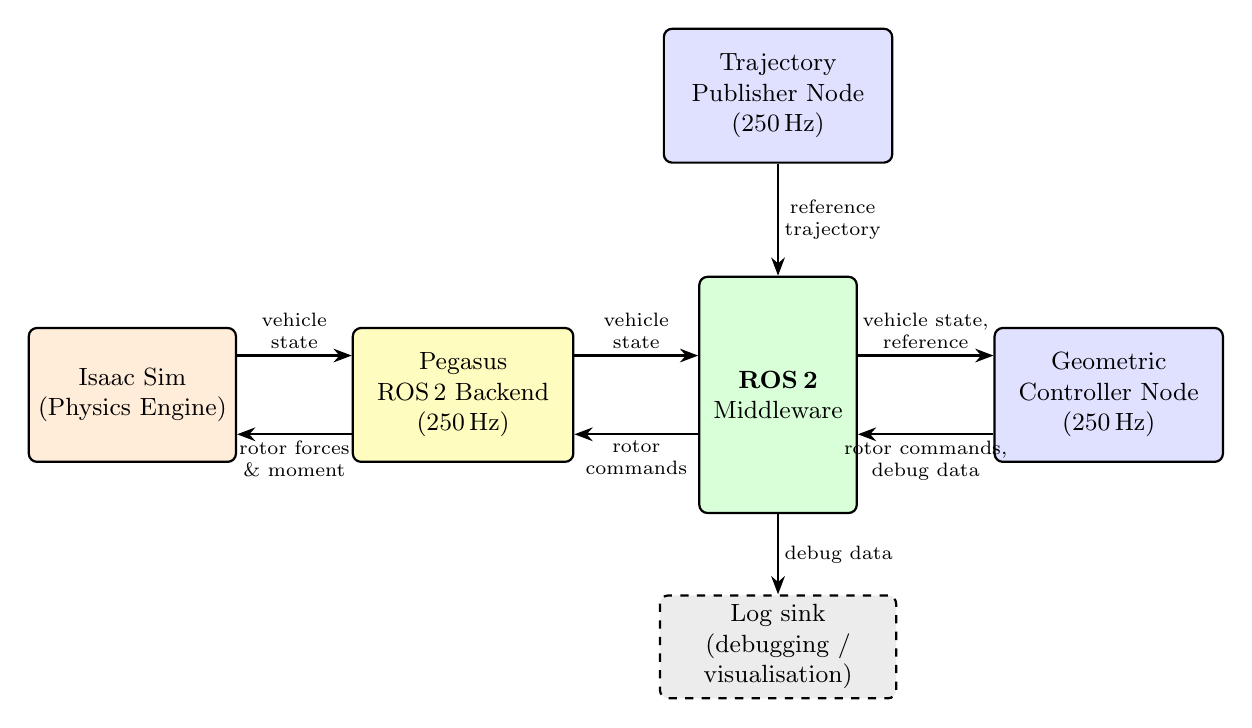
\begin{tikzpicture}[
    font=\small,
    sim/.style={draw, thick, minimum height=1.7cm, minimum width=2.4cm, align=center,
                fill=orange!15, rounded corners=3pt},
    backend/.style={draw, thick, minimum height=1.7cm, minimum width=2.8cm, align=center,
                    fill=yellow!25, rounded corners=3pt},
    ros2/.style={draw, thick, minimum height=3cm, minimum width=2cm, align=center,
                 fill=green!15, rounded corners=3pt},
    pynode/.style={draw, thick, minimum height=1.7cm, minimum width=2.9cm, align=center,
                   fill=blue!12, rounded corners=3pt},
    logsink/.style={draw, thick, dashed, minimum height=1.3cm, minimum width=3cm, align=center,
                    fill=gray!15, rounded corners=3pt},
    arr/.style={->, >=Stealth, thick},
    elab/.style={font=\scriptsize, align=center, inner sep=2pt}
]

% Main horizontal spine
\node[sim]     (isaac)   at (0, 0)    {Isaac Sim\\(Physics Engine)};
\node[backend] (backend) at (4.2, 0)  {Pegasus\\ROS\,2 Backend\\(250\,Hz)};
\node[ros2]    (ros2)    at (8.2, 0)  {\textbf{ROS\,2}\\Middleware};
\node[pynode]  (ctrl)    at (12.4, 0) {Geometric\\Controller Node\\(250\,Hz)};

% Trajectory publisher above, log sink below
\node[pynode]  (traj)    at (8.2, 3.8)  {Trajectory\\Publisher Node\\(250\,Hz)};
\node[logsink] (logs)    at (8.2, -3.2) {Log sink\\(debugging /\\visualisation)};

% Isaac Sim <-> Pegasus Backend (direct Python API, not ROS)
\draw[arr] ([yshift=5mm]isaac.east) -- node[above, elab]{vehicle\\state}
    ([yshift=5mm]backend.west);
\draw[arr] ([yshift=-5mm]backend.west) -- node[below, elab]{rotor forces\\\& moment}
    ([yshift=-5mm]isaac.east);

% Pegasus Backend <-> ROS 2
\draw[arr] ([yshift=5mm]backend.east) -- node[above, elab]{vehicle\\state}
    ([yshift=5mm]ros2.west);
\draw[arr] ([yshift=-5mm]ros2.west) -- node[below, elab]{rotor\\commands}
    ([yshift=-5mm]backend.east);

% ROS 2 <-> Geometric Controller
\draw[arr] ([yshift=5mm]ros2.east) -- node[above, elab]{vehicle state,\\reference}
    ([yshift=5mm]ctrl.west);
\draw[arr] ([yshift=-5mm]ctrl.west) -- node[below, elab]{rotor commands,\\debug data}
    ([yshift=-5mm]ros2.east);

% Trajectory Publisher --> ROS 2
\draw[arr] (traj.south) -- node[right, elab]{reference\\trajectory} (ros2.north);

% ROS 2 --> Log sink
\draw[arr] (ros2.south) -- node[right, elab]{debug data} (logs.north);

\end{tikzpicture}
\caption{ROS\,2 system architecture of the closed-loop simulation. The ROS\,2 middleware (green, centre) mediates all inter-node publish/subscribe communication; the only direct link is between Isaac Sim and the Pegasus backend, which are coupled via Isaac Sim's Python API rather than ROS topics. The backend pulls the vehicle state from Isaac Sim at $250$~Hz and republishes it on ROS topics (\texttt{state/pose}, \texttt{state/twist}, \texttt{state/twist\_inertial}, \texttt{state/accel}, \texttt{state/jerk}); conversely, it converts the normalised-throttle commands received on \texttt{control/rotor\{i\}/ref} into per-rotor forces applied to the rotor links and a reactive rolling moment applied to the body, before passing them to Isaac Sim. The trajectory publisher emits the flat-output references on \texttt{trajectory/desired/*} (position through snap and yaw through yaw-acceleration). The geometric controller subscribes to both the state and the reference topics, outputs four normalised-throttle commands on \texttt{control/rotor\{i\}/ref}, and publishes internal controller variables and outputs on \texttt{control/internal/*} and \texttt{control/output/*} for offline analysis. All three ROS\,2 nodes run at $250$~Hz, matched to the Isaac Sim physics step.}
\label{fig:block-diagram}
\end{figure}

\subsection{Controller Parameter Tuning}
Separate gains were used for the yaw axis so that the yaw response could be tuned independently of the roll/pitch response. The gains used for all simulation results in Section~\ref{sec:results} are listed in Table~\ref{tab:gains}. The outer-loop position gains were tuned first with an approximate damping ratio of $\zeta \approx 0.7$, then the inner-loop attitude gains were chosen to give a roughly $10\!:\!1$ bandwidth separation. The yaw gains are smaller because yaw tracking is less time-critical and the $z$-axis has a larger inertia.

\begin{table}[H]
    \centering
    \caption{Controller gains used for all trajectory tests.}
    \label{tab:gains}
    \begin{tabular}{lcl}
        \toprule
        Parameter        & Value  & Description \\
        \midrule
        $k_x$            & $1.0$  & Position gain \\
        $k_v$            & $1.7$  & Velocity gain \\
        $k_R$            & $1.5$  & Roll/pitch attitude gain \\
        $k_\Omega$       & $0.4$  & Roll/pitch rate gain \\
        $k_{R,\psi}$     & $1.0$  & Yaw attitude gain \\
        $k_{\Omega,\psi}$& $0.35$ & Yaw rate gain \\
        Publish rate     & $250$~Hz & Control loop frequency \\
        \bottomrule
    \end{tabular}
\end{table}

% ============================================================
\section{Simulation Results}
\label{sec:results}
% ============================================================

The tuned controller was validated in Isaac Sim on four reference trajectories. For each test, the controller ran at 250~Hz, the trajectory publisher at 250~Hz, and the Isaac Sim physics step at 250~Hz. A consistent set of plots was generated for every run: 3D trajectory path, per-axis position tracking, roll/pitch/yaw tracking, position and attitude tracking errors, and rotor throttle commands. For brevity, representative plots are shown below; the complete plot set for every trajectory is provided in the accompanying data package.

\subsection{Test 1 --- Hover}
The quadrotor takes off from the ground and tracks a fixed hover setpoint at $[0,0,1]^\top$~m. This is the simplest test and exercises only the translational channel under quasi-static conditions.

\begin{figure}[H]
    \centering
    \begin{subfigure}{0.48\textwidth}
        
\includegraphics[width=\linewidth]{figures/hover/tracking_xyz.png}
        \caption{Position tracking.}
    \end{subfigure}
    \hfill
    \begin{subfigure}{0.48\textwidth}
        
\includegraphics[width=\linewidth]{figures/hover/error_position.png}
        \caption{Position error.}
    \end{subfigure}
    \caption{Hover test. The quadrotor rises from the ground and settles at $z = 1$~m with negligible steady-state error.}
    \label{fig:hover}
\end{figure}

\subsection{Test 2 --- Circle}
Starting from a hover at $[0,0,1]^\top$~m, the quadrotor tracks a planar circle of radius $2$~m at $\omega = 0.5$~rad/s for three complete cycles. The yaw reference follows the tangent of the circle, exercising all four channels.

\begin{figure}[H]
    \centering
    \begin{subfigure}{0.48\textwidth}
        
\includegraphics[width=\linewidth]{figures/circle/path_xy.png}
        \caption{Top-down trajectory.}
    \end{subfigure}
    \hfill
    \begin{subfigure}{0.48\textwidth}
        
\includegraphics[width=\linewidth]{figures/circle/tracking_xyz.png}
        \caption{Per-axis position tracking.}
    \end{subfigure}
    \caption{Planar circle of radius $2$~m at $\omega = 0.5$~rad/s. Three complete cycles are tracked with a small lag inherent to the finite controller bandwidth.}
    \label{fig:circle}
\end{figure}

\begin{figure}[H]
    \centering
    \begin{subfigure}{0.48\textwidth}
        
\includegraphics[width=\linewidth]{figures/circle/error_position.png}
        \caption{Position error.}
    \end{subfigure}
    \hfill
    \begin{subfigure}{0.48\textwidth}
        
\includegraphics[width=\linewidth]{figures/circle/error_attitude.png}
        \caption{Attitude error.}
    \end{subfigure}
    \caption{Tracking errors for the circle trajectory.}
    \label{fig:circle-errors}
\end{figure}

\subsection{Test 3 --- Figure-Eight}
Starting from a hover, the quadrotor traces a planar lemniscate with $x_d = r\sin(\omega t)$ and $y_d = (r/2)\sin(2\omega t)$, with $r = 2$~m and $\omega = 0.5$~rad/s. This trajectory is more demanding than the circle because the velocity and acceleration profiles are non-stationary and the aircraft must pass through zero yaw twice per cycle.

\begin{figure}[H]
    \centering
    \begin{subfigure}{0.48\textwidth}
        
\includegraphics[width=\linewidth]{figures/figure_eight/path_xy.png}
        \caption{Top-down trajectory.}
    \end{subfigure}
    \hfill
    \begin{subfigure}{0.48\textwidth}
        
\includegraphics[width=\linewidth]{figures/figure_eight/error_position.png}
        \caption{Position error.}
    \end{subfigure}
    \caption{Planar figure-eight trajectory. The characteristic double-loop shape is reproduced accurately.}
    \label{fig:figure-eight}
\end{figure}

\subsection{Test 4 --- Ascending Elliptic Helix}
The quadrotor takes off from the ground and follows an elliptic helix with semi-axes $a = 1$~m and $b = 2$~m, a climb rate of $0.1$~m/s, and a rotation rate of $0.5$~rad/s for three cycles. This trajectory exercises all six degrees of freedom simultaneously.

\begin{figure}[H]
    \centering
    \begin{subfigure}{0.48\textwidth}
        
\includegraphics[width=\linewidth]{figures/elliptic_helix/path_xyz_3d.png}
        \caption{3D path.}
    \end{subfigure}
    \hfill
    \begin{subfigure}{0.48\textwidth}
        
\includegraphics[width=\linewidth]{figures/elliptic_helix/tracking_xyz.png}
        \caption{Per-axis position tracking.}
    \end{subfigure}
    \caption{Ascending elliptic helix. The aircraft spirals upward while yawing with the trajectory.}
    \label{fig:helix}
\end{figure}

\begin{figure}[H]
    \centering
    \begin{subfigure}{0.48\textwidth}
        
\includegraphics[width=\linewidth]{figures/elliptic_helix/error_position.png}
        \caption{Position error.}
    \end{subfigure}
    \hfill
    \begin{subfigure}{0.48\textwidth}
        
\includegraphics[width=\linewidth]{figures/elliptic_helix/control_thrust.png}
        \caption{Collective thrust command.}
    \end{subfigure}
    \caption{Helix tracking error and collective-thrust command. The thrust stays well within the saturation limit and settles to the weight of the aircraft once the aircraft reaches the final hover at the end of the trajectory.}
    \label{fig:helix-errors}
\end{figure}

\subsection{Discussion}
Across all four trajectories, the controller achieves sub-decimetre position tracking and sub-$5^\circ$ attitude tracking under rich time-varying references. The steady-state position error on the hover test is dominated by the small residual offset between the CAD-estimated CoG and the actual simulated CoG, rather than by the controller itself. A short transient at the start of each trajectory is visible in the error plots; this is the expected exponential decay from the initial condition predicted by Propositions~\ref{prop:1}--\ref{prop:3}. Rotor throttle commands stay within the $[0,1]$ saturation bounds throughout, confirming that the chosen trajectories are dynamically feasible for the F450.

% ============================================================
\section{Conclusion and Future Work}
\label{sec:conclusion}
% ============================================================

\subsection{Conclusion}
This project delivered a complete pipeline from CAD modelling through to validated closed-loop simulation of an F450 quadrotor under geometric tracking control on $\se$. The CAD-derived vehicle model, the linear thrust identification, a self-contained treatment of the geometric-control stability proofs, the analytical feed-forward derivation, and the Pegasus/ROS\,2 integration together form a reusable basis for future controller development in the FSC Lab. The controller was shown to track hover, circle, figure-eight, and helix references with low error.

\subsection{Future Work}
\label{sec:future-work}
Several directions build naturally on this work:
\begin{itemize}
    \item \textbf{Accurate rotor-moment identification.} The rolling-moment coefficient $k_m$ was estimated from manufacturer data and should be measured directly on a torque bench.
    \item \textbf{Disturbance rejection.} Adding an integral term or a disturbance observer to the geometric controller would compensate for the residual CoG offset and modelling errors that limit steady-state accuracy.
    \item \textbf{Aggressive manoeuvres.} The region of attraction of Propositions~\ref{prop:1}--\ref{prop:3} is almost global; flips and large-angle recovery tests were not exercised in this project and would demonstrate the controller's full capability.
    \item \textbf{Hardware deployment.} The controller is implemented in ROS\,2 and is directly portable to the FSC Lab F450 once a state-estimator (e.g.\ motion-capture or VIO) is connected to the same topics used in simulation.
    \item \textbf{Adaptive control.} Lee et al.'s adaptive extension accounts for unknown mass and inertia and would be a natural next step.
\end{itemize}

% ============================================================
\begin{thebibliography}{9}
\bibitem{Lee2010CDC}
T.~Lee, M.~Leok, and N.~H.~McClamroch,
``Geometric tracking control of a quadrotor UAV on $\mathrm{SE}(3)$,''
in \emph{Proc.\ IEEE Conf.\ Decision and Control (CDC)}, 2010, pp.\ 5420--5425.

\bibitem{Pegasus}
M.~Jacinto, J.~Pinto, J.~Patrikar, J.~Keller, R.~Cunha, S.~Scherer, and A.~Pascoal,
``Pegasus Simulator: An Isaac Sim framework for multiple aerial vehicles simulation,''
\emph{arXiv preprint arXiv:2307.05263}, 2023.

\bibitem{IsaacSim}
NVIDIA Corporation, \emph{Isaac Sim}, \url{https://developer.nvidia.com/isaac-sim}.

\bibitem{ROS2}
Open Robotics, \emph{ROS\,2 Documentation}, \url{https://docs.ros.org/en/humble/}.

\bibitem{Mellinger2011}
D.~Mellinger and V.~Kumar,
``Minimum snap trajectory generation and control for quadrotors,''
in \emph{Proc.\ IEEE Int.\ Conf.\ Robotics and Automation (ICRA)}, 2011, pp.\ 2520--2525.
\end{thebibliography}

\end{document}